%%%%%%%%%%%%%%%%
%% RESULTADOS %%
%%%%%%%%%%%%%%%%

\section{Resultados}
\lipsum[1]

\begin{table}[h]
	\caption{Sample Basic Table}
	\label{tab:BasicTable}
	\begin{tabular}{@{}llr@{}}         \toprule
		\multicolumn{2}{c}{Item}        \\ \cmidrule(r){1-2}
		Animal    & Description & Price \\ \midrule
		Gnat      & per gram    & 13.65 \\
		& each        &  0.01 \\
		Gnu       & stuffed     & 92.50 \\
		Emu       & stuffed     & 33.33 \\
		Armadillo & frozen      &  8.99 \\ \bottomrule
	\end{tabular}
\end{table}

\lipsum[1]

\begin{figure}
	\caption{Descripción de figuras.}
	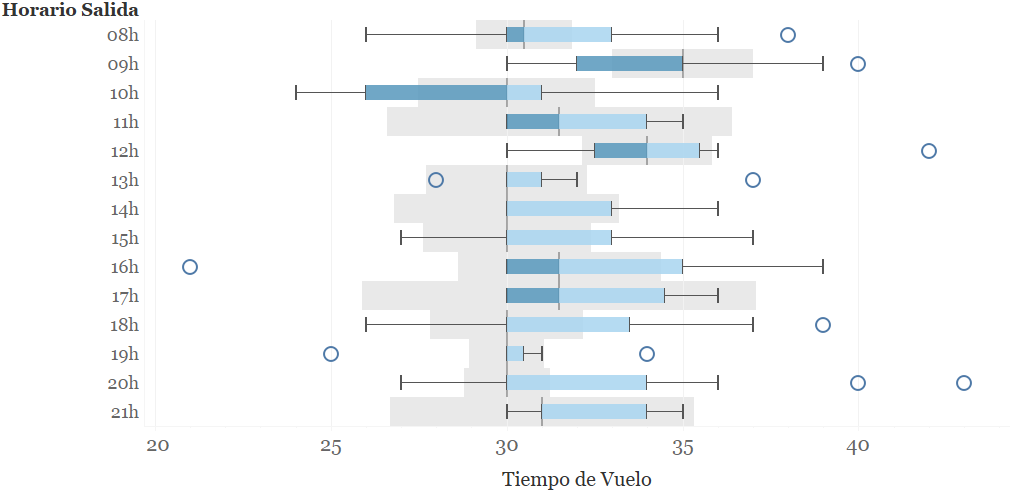
\includegraphics[scale=0.85]{contenido/multimedios/figura1}
	\label{fig:Figure1}
\end{figure}

\lipsum[2]

\begin{table}[h]
	\begin{threeparttable}
	  \caption{A More Complex Decked Table}
	  \label{tab:DeckedTable}
	  \begin{tabular}{@{}lrrr@{}}         \toprule
	  Distribution type  & \multicolumn{2}{l}{Percentage of} & Total number   \\
						 & \multicolumn{2}{l}{targets with}  & of trials per  \\
						 & \multicolumn{2}{l}{segment in}    & participant    \\ \cmidrule(r){2-3}
									  &  Onset  &  Coda            &          \\ \midrule
	  Categorical -- onset\tabfnm{a}  &    100  &     0            &  196     \\
	  Probabilistic                   &     80  &    20\tabfnm{*}  &  200     \\
	  Categorical -- coda\tabfnm{b}   &      0  &   100\tabfnm{*}  &  196     \\ \midrule
	  \end{tabular}
	  \tablenote{All data are approximate.
  
			  \tabfnt{a}Categorical may be onset.
			  \tabfnt{b}Categorical may also be coda.
  
			  \tabfnt{*}\textit{p} < .05.
			  \tabfnt{**}\textit{p} < .01.
		   }
	\end{threeparttable}
  \end{table}
\lipsum[1]